\newpage
\section{Classification Models (Trainable Vectorization and Emebddings)}
La clasificación de los modelos en conjunto con su vectorización y los \textit{embeddings} inicia con la búsqueda de los mejores hiper parámetros mediante una búsqueda de grilla modificada. En un principio, la búsqueda de grilla debería variar una serie de hiper parámetros con el fin de encontrar los que producen un mejor modelo. Sin embargo, variar todos los parámetros dentro de una misma búsqueda implica entrenar y evaluar múltiples modelos, lo cual requiere una gran cantidad de tiempo y recursos computacionales. Con el fin de disminuir el tiempo dedicado a la búsqueda de los hiper parámetros se realiza una búsqueda de cada valor de forma independiente. Esta aproximación se ve favorecida por el conocimiento previo del problema y de algunos valores obtenidos en etapas previas del desarrollo del problema.

La búsqueda de los hiper parámetros se hace variando los valores correspondientes a la dimensionalidad del embedding, la longitud de las sentencias y el tamaño del vocabulario. El orden en el cual se realiza esta búsqueda está determinado por el hecho de que se conocen datos de la longitud de las sentencias y del tamaño del vocabulario. En este sentido, el primer parámetro a buscar corresponde a la dimensionalidad del embedding, seguido de la longitud de las sentencias y finalizando con el tamaño del vocabulario. Vale la pena mencionar que otras condiciones relacionadas a los modelos, como lo son instancias de regularización y variaciones en la vectorización, van a ser evaluadas posteriormente.

Para realizar la búsqueda de los parámetros se utiliza un modelo, descrito en la tabla \ref{tab:deep_em_hyper_params}, de una red neuronal completamente conectada (FCN, \textit{Fully Connected Network}). La primera capa de la red corresponde a la de vectorización de texto que oficia como entrada al modelo, recibiendo las sentencias a clasificar. La salida de la capa de vectorización corresponde a una secuencia con una cantidad dada de tokens denotados por \textit{seq\_len}. Una vez se ha vectorizado el texto, este entra a la capa de embedding cuya dimensionalidad va a estar dada por \textit{seq\_len} y \textit{embedding\_dim} que representa la dimensionalidad del embedding. La capa de embedding presenta una salida de dos dimensiones que debe ser ajustada para alimentar las capas densas de la red neuronal. Para dicho ajuste se usa una capa que calcula el promedio global de cada embedding, convirtiendo así la salida de dos dimensiones en un vector con \textit{embedding\_dim} dimensiones. La capa densa de la red contienen un número de neuronas que se calcula con el promedio entre \textit{embedding\_dim} y \textit{output\_dim}, que corresponde al número de clases que serán clasificadas. Finalmente, la última capa contiene \textit{output\_dim} neuronas con el fin de realizar la clasificación correspondiente.

\begin{table}[h]
    \centering
    \begin{tabular}{|l|l|}
        \hline
        \textbf{Tipo de Capa} & \textbf{Características} \\ \hline
        Vectorización de Texto & Denotada por \textit{seq\_len} \\ \hline
        Embedding & Denotada por \textit{seq\_len} y \textit{embedding\_dim} \\ \hline
        Promedio Global de 1D & Convierte los valores a una dimensión \\ \hline
        Densa & Neuronas: promedio entre \textit{embedding\_dim} y \textit{output\_dim} \\ \hline
        Densa & Neuronas: dado por \textit{output\_dim} \\ \hline
    \end{tabular}
    \caption{Definición del modelo para la evaluación y selección de hiper parámetros.}
    \label{tab:deep_em_hyper_params}
\end{table}

La primera etapa de la búsqueda de hiper parámetros se dedicó a fijar la dimensionalidad del embedding. Las posibles dimensiones consideradas fueron de 5, 10, 15, 20, 25, 50, 100 y 150. Las figuras \ref{fig:em_embedding_simpsons} y \ref{fig:em_embedding_friends} presentan respectivamente los resultados para los dos conjuntos de datos: el de \textit{Los Simpsons} y \textit{Friends}. Se puede identificar que los mejores resultados se obtienen con una dimensión de 150 para los dos conjuntos de datos. Vale la pena notar que los modelos para el conjunto de datos de \textit{Friends} demuestran aprendizaje, pero con bajos niveles de recall. 

\begin{figure}
    \centering
    \begin{subfigure}[b]{0.45\textwidth}
        \centering
        \includegraphics[width=\textwidth]{doc/images/embeddings/simpsons.pdf}
        \caption{Métricas de evaluación para diferentes dimensiones del embedding en el conjunto de datos de \textit{Los Simpsons}.}
        \label{fig:em_embedding_simpsons}
    \end{subfigure}
    \hfill
    \begin{subfigure}[b]{0.45\textwidth}
        \centering
        \includegraphics[width=\textwidth]{doc/images/embeddings/friends.pdf}
        \caption{Métricas de evaluación para diferentes dimensiones del embedding en el conjunto de datos de \textit{Friends}.}
        \label{fig:em_embedding_friends}
    \end{subfigure}
    \caption{Métricas de evaluación para la búsqueda de la mejor dimensión del embedding.}
    \label{fig:em_embedding}
\end{figure}

Una vez se ha definido la mejor dimensión para el embedding, se procede a evaluar distintas longitudes de las secuencias. Siguiendo un procedimiento similar al usado para las dimensiones del embedding, se define una serie de posibles longitudes para las secuencias. En este caso las longitudes consideradas fueron: 5, 10, 15, 20, 25, 50 y 100. Los resultados de esta búsqueda se presentan en la figura \ref{fig:em_seq_len}.


\begin{figure}
    \centering
    \begin{subfigure}[b]{0.45\textwidth}
        \centering
        \includegraphics[width=\textwidth]{doc/images/seq_len/simpsons.pdf}
        \caption{Métricas de evaluación para diferentes longitudes de las secuencias en el conjunto de datos de \textit{Los Simpsons}.}
        \label{fig:em_seq_len_simpsons}
    \end{subfigure}
    \hfill
    \begin{subfigure}[b]{0.45\textwidth}
        \centering
        \includegraphics[width=\textwidth]{doc/images/seq_len/friends.pdf}
        \caption{Métricas de evaluación para diferentes longitudes de las secuencias en el conjunto de datos de \textit{Friends}.}
        \label{fig:em_seq_len_friends}
    \end{subfigure}
    \caption{Métricas de evaluación para la búsqueda de la mejor longitud de secuencia.}
    \label{fig:em_seq_len}
\end{figure}


\subsection{Simpsons Dataset}

\subsection{Friends Dataset}

